\begin{frontmatter}
    \begin{highlights}
    \item Classical VQPM: for QUBO problems every VQPM measurement shot, and hence every qubit-locking decision, can be sampled classically at $O(n^2)$ cost per shot.
    \item To first order the VQPM update is mirror descent on the mean energy of a product distribution; locking reads the signs of this update and speeds it up without steering it toward the optimum.
    \item Without locking, VQPM finds the optimum as often as QAOA with a good optimizer up to $n=16$, but needs about 100 times more iterations than with locking.
    \item Up to $n=100$, the success rate of VQPM falls to 0.24 without locking and to at most 0.05 with locking, while simulated annealing stays near 0.98.
    \item On a device, VQPM needs $10^5$ to $10^6$ shots per iteration and a locking threshold below the level at which noise holds the probability differences.
    \end{highlights}
\begin{graphicalabstract}
%\documentclass[tikz,border=3mm]{standalone}
\usetikzlibrary{positioning, shapes, arrows.meta, calc, decorations.pathreplacing}
%\usepackage{emoji}

%\begin{document}
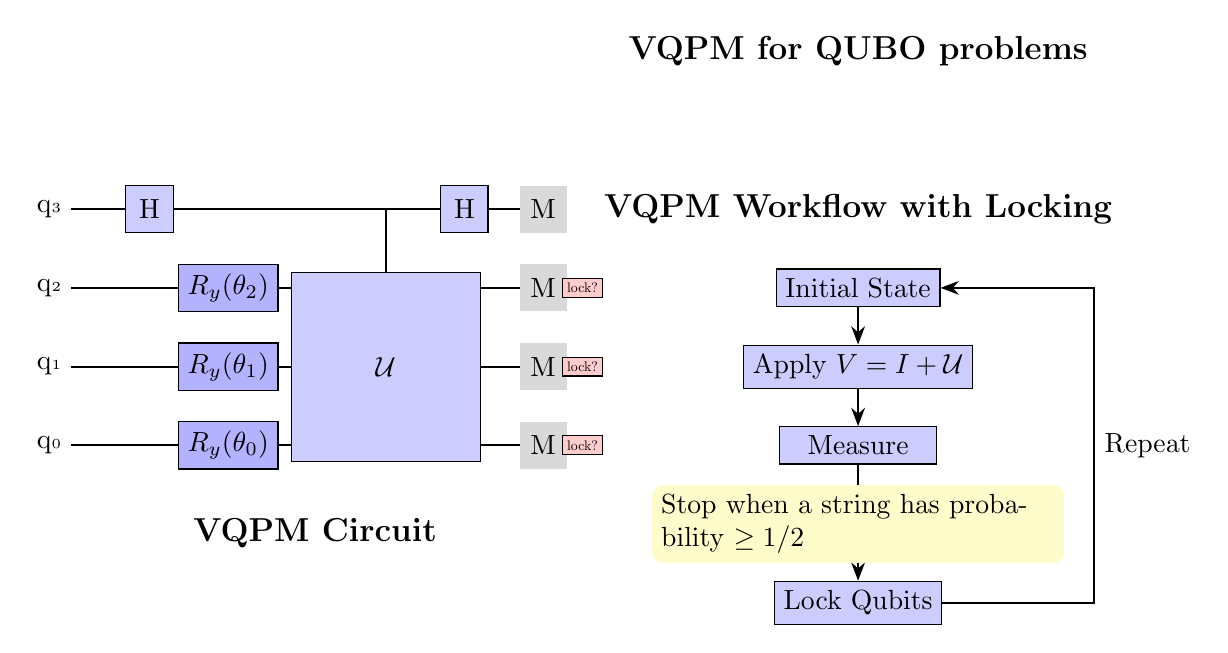
\begin{tikzpicture}[
    node distance=5mm,
    title/.style={font=\large\bfseries},
    circuit/.style={draw,thick,minimum width=3cm,minimum height=1.5cm},
    qgate/.style={draw,fill=blue!20,minimum size=6mm},
      Ugate/.style={draw,fill=blue!20,minimum size=24mm},
    measure/.style={fill=gray!30,shape=rectangle,minimum size=6mm},
    arrow/.style={-Stealth,thick},
    highlight/.style={fill=yellow!20,rounded corners}
]

% Left panel - VQPM Circuit
\begin{scope}[local bounding box=left]
    % Qubit lines
    \foreach \y in {0,1,2,3} {
        \draw[thick] (0,\y) -- (6,\y);
        \node[left] at (0,\y) {q\tiny{\y}};
    }
    
    % Circuit elements
    \node[qgate] (h0) at (1,3) {H};
    \node[qgate] (h1) at (5,3) {H};
    \node[measure] (m0) at (6,3) {M};
    \node[Ugate] (crz) at (4,1) {$\mathcal{U}$};
    \draw[thick]  (4,3) -- (crz);
    \foreach \y in {0,1,2} {
        \node[qgate,fill=blue!30] (ry\y) at (2,\y) {$R_y(\theta_{\y})$};
        \node[measure] (m\y) at (6,\y) {M};
    }
    
    % Lock icons
    \foreach \y in {0,1,2} {
        \node[draw,fill=red!20,scale=0.5] at ($(m\y)+(0.5,0)$) {lock?};
    }
    
    \node[title,below=0.5cm of left] {VQPM Circuit};
\end{scope}

% Center panel - Workflow
\begin{scope}[local bounding box=center,xshift=10cm, yshift=3cm]
    \node[title] (workflow) {VQPM Workflow with Locking};
    
    \node[draw,fill=blue!20,minimum width=2cm] (init) at (0,-1) {Initial State};
    \node[draw,fill=blue!20,minimum width=2cm] (apply) at (0,-2) {Apply $V = I+\mathcal{U}$};
    \node[draw,fill=blue!20,minimum width=2cm] (measure) at (0,-3) {Measure};
    \node[draw,fill=blue!20,minimum width=2cm] (lock) at (0,-5) {Lock Qubits};
    
    \draw[arrow] (init) -- (apply);
    \draw[arrow] (apply) -- (measure);
    \draw[arrow] (measure) -- (lock);
    \draw[arrow] (lock) -- ++(3,0) |- node[pos=0.25,right] {Repeat} (init);
    
    \node[highlight, text width=5cm] at (0,-4) {Stop when a string has probability $\ge 1/2$};
\end{scope}

% Title
\node[title] at (10,5) 
    {VQPM for QUBO problems};

\end{tikzpicture}
%\end{document}
\end{graphicalabstract}
\end{frontmatter}
